% This LaTeX was auto-generated from MATLAB code.
% To make changes, update the MATLAB code and export to LaTeX again.

\documentclass{article}

\usepackage[utf8]{inputenc}
\usepackage[T1]{fontenc}
\usepackage{lmodern}
\usepackage{graphicx}
\usepackage{color}
\usepackage{hyperref}
\usepackage{amsmath}
\usepackage{amsfonts}
\usepackage{epstopdf}
\usepackage[table]{xcolor}
\usepackage{matlab}

\sloppy
\epstopdfsetup{outdir=./}
\graphicspath{ {./TemperaturRegulering_images/} }

\begin{document}

\matlabtitle{\textbf{Desig af temperatur regulering}}


\vspace{1em}

\vspace{1em}
\begin{matlabcode}
clear all
close all 
clc
s=tf('s')
\end{matlabcode}
\begin{matlaboutput}
s =
 
  s
 
Continuous-time transfer function.
\end{matlaboutput}



\vspace{1em}
\begin{par}
\begin{flushleft}
\textbf{Målt data (wostcase) }
\end{flushleft}
\end{par}

\begin{par}
\begin{flushleft}
Tilføjelse af 750 ml væske af 21 grader, i 22 litter akvarie vand på 30 grader
\end{flushleft}
\end{par}

\begin{matlabcode}
load Step_Maaling_af_30_grader_tilsat_21_grader.txt

Ts_sensor = 17.76;
fs_sensor = 1/Ts_sensor
\end{matlabcode}
\begin{matlaboutput}
fs_sensor = 0.0563
\end{matlaboutput}
\begin{matlabcode}

t_akse_koldt_vand = (1:length(Step_Maaling_af_30_grader_tilsat_21_grader))*(1/fs_sensor);

plot(t_akse_koldt_vand,Step_Maaling_af_30_grader_tilsat_21_grader)
title('Tilsætning af 750 ml vand på 21 grader, i 22 liter vand på 30 grader')
ylim([28 30.5])
xlim([0 500])
xlabel('Tid [s]')
ylabel('Tempertur [C{\circ}]')
\end{matlabcode}
\begin{center}
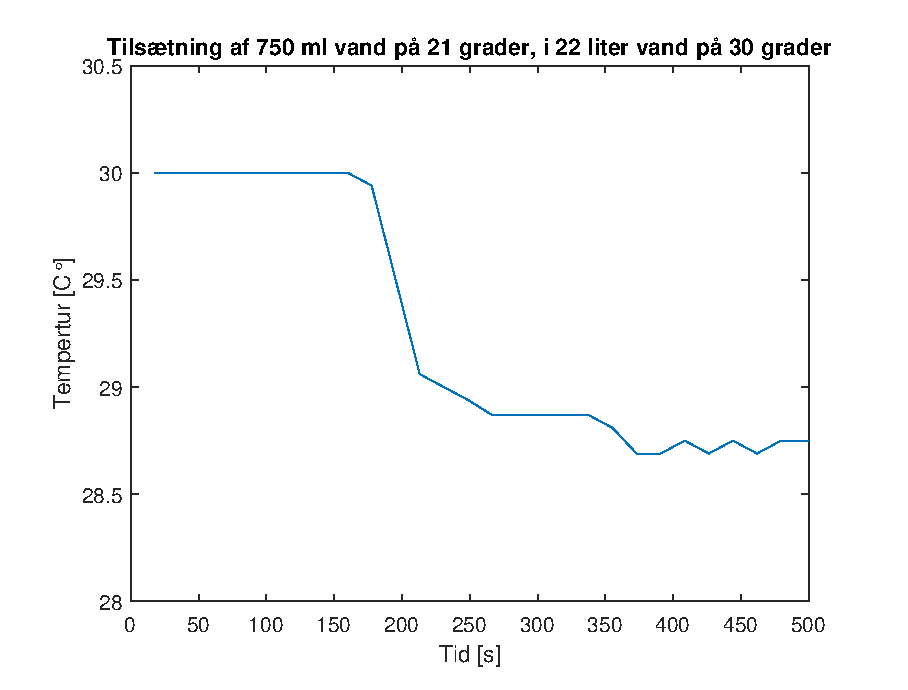
\includegraphics[width=\maxwidth{56.196688409433015em}]{figure_0.eps}
\end{center}



\vspace{1em}
\begin{par}
\begin{flushleft}
\textbf{Målt data (Proces)}
\end{flushleft}
\end{par}

\begin{par}
\begin{flushleft}
Stepresopons for 120 Watt varmelegeme. 20\% dutycycle
\end{flushleft}
\end{par}

\begin{matlabcode}
load 'WaterHeated.mat'
step_respons_temp = WaterHeated_Fake(350:1419);
t_akse_step = (1:length(step_respons_temp))*(1/fs_sensor);
plot(t_akse_step,step_respons_temp)
hold on
\end{matlabcode}


\vspace{1em}
\begin{par}
\begin{flushleft}
\textbf{Åbensløjfe-krakterstik (Proces)}
\end{flushleft}
\end{par}

\begin{matlabcode}
offset = 22.3 %stuetemperatur
\end{matlabcode}
\begin{matlaboutput}
offset = 22.3000
\end{matlaboutput}
\begin{matlabcode}
input = 20 %procent duty cycle
\end{matlabcode}
\begin{matlaboutput}
input = 20
\end{matlaboutput}
\begin{matlabcode}
output = 25.19-offset %vand Temperatur
\end{matlabcode}
\begin{matlaboutput}
output = 2.8900
\end{matlaboutput}

\begin{par}
\begin{flushleft}
Type : 2 ordens
\end{flushleft}
\end{par}

\begin{par}
\begin{flushleft}
Zeta: 0.85
\end{flushleft}
\end{par}

\begin{par}
\begin{flushleft}
Settletime Tsettle  = 16000 s
\end{flushleft}
\end{par}

\begin{par}
\begin{flushleft}
wBW (båndbredde) = Wn (naturlige frekvens)
\end{flushleft}
\end{par}

\begin{matlabcode}
zeta = 0.85;
Tsettle = 16000
\end{matlabcode}
\begin{matlaboutput}
Tsettle = 16000
\end{matlaboutput}
\begin{matlabcode}
wBW=(4/(zeta*Tsettle))*sqrt((1-2*zeta^2)+sqrt(4*zeta^4-4*zeta^2+2)) 
\end{matlabcode}
\begin{matlaboutput}
wBW = 2.3704e-04
\end{matlaboutput}
\begin{matlabcode}
DC_gain=output/input
\end{matlabcode}
\begin{matlaboutput}
DC_gain = 0.1445
\end{matlaboutput}
\begin{matlabcode}

Gp=(DC_gain*(wBW^2))/(s^2+s*2*zeta*wBW+wBW^2)
\end{matlabcode}
\begin{matlaboutput}
Gp =
 
           8.119e-09
  ----------------------------
  s^2 + 0.000403 s + 5.619e-08
 
Continuous-time transfer function.
\end{matlaboutput}
\begin{matlabcode}

step(input*Gp+offset,'red')
legend('Mesured','Model','location','southeast')
title 'Steprespons for varmelegeme, 20% duty cycle'
ylabel('Tempertur [C{\circ}]')
xlabel('Tid')
ylim([22 25.5])
hold off
\end{matlabcode}
\begin{center}
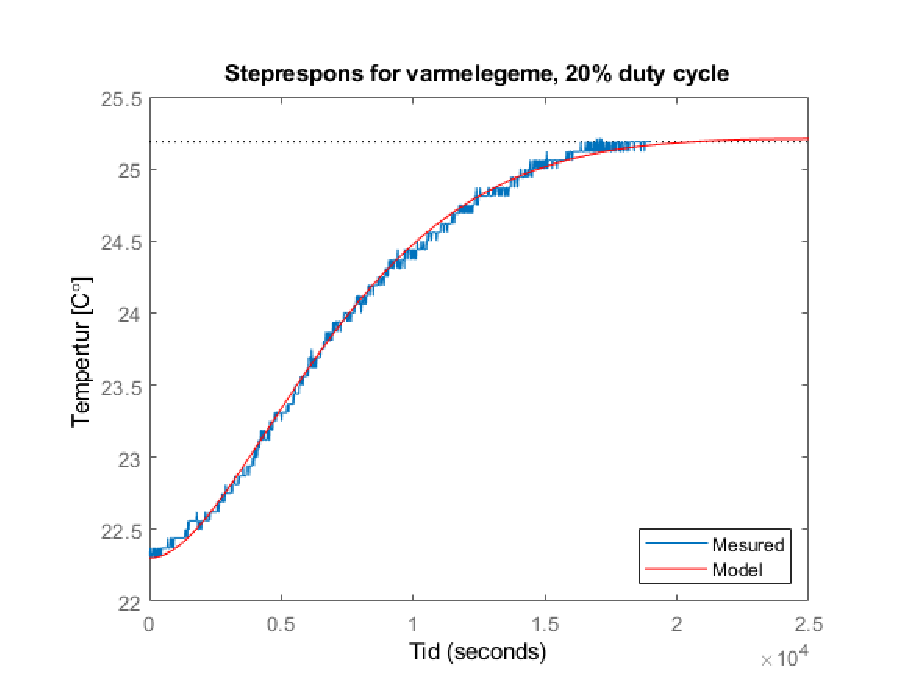
\includegraphics[width=\maxwidth{56.196688409433015em}]{figure_1.eps}
\end{center}



\vspace{1em}
\begin{par}
\begin{flushleft}
\textbf{Regulerings begrænsninger}
\end{flushleft}
\end{par}

\begin{par}
\begin{flushleft}
Systet er begrænset af en dytycycle fra 0 - 100\%. Det vil sige systemte skal designet med mente at regulatorern ALDRIG vil forsøge at levere et output(dutycycle) til processen(Varmelegeme og vand) uden for begrændsningerne.
\end{flushleft}
\end{par}

\begin{par}
\begin{flushleft}
Worst case siturationen (Tilføjelse af 750 ml væske, af 21 grader, i 22 litter akvarievand af 30 grader) giver et temperaturfald på 1.2 grader.
\end{flushleft}
\end{par}

\begin{par}
\begin{flushleft}
Derfor defineres steppet systemet skal kunne håndtere.
\end{flushleft}
\end{par}

\begin{par}
\begin{flushleft}
\textbf{step = 1.2} \textit{28.8 -\textgreater{} 30 grader}
\end{flushleft}
\end{par}

\begin{par}
\begin{flushleft}
\textbf{Grader offset = 28.8}
\end{flushleft}
\end{par}

\begin{par}
\begin{flushleft}
\textbf{Dutycycle offset = 45\%}  \textit{(28.8 grader i duty cycle)}
\end{flushleft}
\end{par}

\begin{par}
\begin{flushleft}
\textbf{Stationær fejl \textless{} 1\%}
\end{flushleft}
\end{par}

\begin{matlabcode}
offset_28grader=28.8
\end{matlabcode}
\begin{matlaboutput}
offset_28grader = 28.8000
\end{matlaboutput}
\begin{matlabcode}
dutycycle_offset = (28.8-22.3)/0.1445
\end{matlabcode}
\begin{matlaboutput}
dutycycle_offset = 44.9827
\end{matlaboutput}


\begin{par}
\begin{flushleft}
Risetiem er pt uden regulering  = 11.000 sekunder
\end{flushleft}
\end{par}

\begin{par}
\begin{flushleft}
Vi designer efter et oversving på 10\% og risetime på 8000 sekunder
\end{flushleft}
\end{par}

\begin{par}
\begin{flushleft}
heraf undersøges det om systmet er istand stil at udføre denne ændring i risetime, uden at gå i mætning, eller om en kortere risetime kan introduceres.
\end{flushleft}
\end{par}

\begin{par}
\begin{flushleft}
\textbf{OS = 10\% -\textgreater{} Cmax = 1.1 -\textgreater{} Zeta 0.55 -\textgreater{} Fasemagen 60}
\end{flushleft}
\end{par}

\begin{par}
\begin{flushleft}
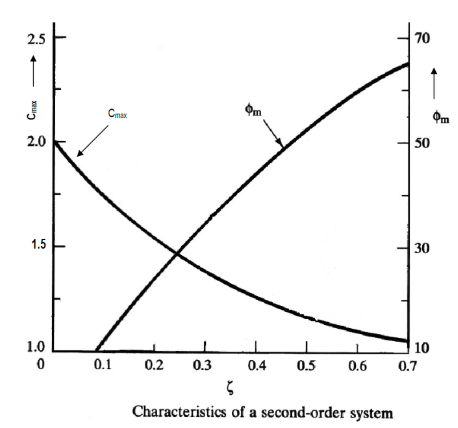
\includegraphics[width=\maxwidth{32.012042147516304em}]{image_0}
\end{flushleft}
\end{par}

\begin{par}
\begin{flushleft}
\textbf{fasemagenfrekvens}
\end{flushleft}
\end{par}

\begin{par}
\begin{flushleft}
Heraf findes en fasemagenfrekvesn der tilsvare zeta værdien på 0.55 og risetime på 8000
\end{flushleft}
\end{par}


\vspace{1em}
\begin{par}
\begin{flushleft}
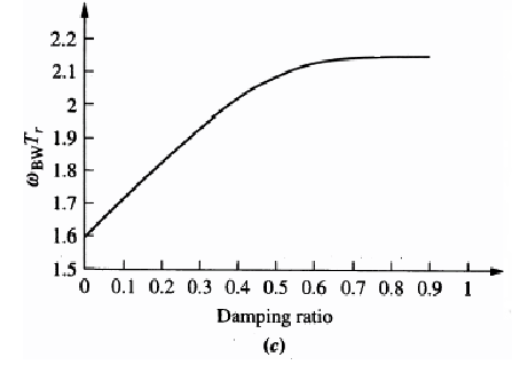
\includegraphics[width=\maxwidth{33.81836427496237em}]{image_1}
\end{flushleft}
\end{par}


\vspace{1em}
\begin{matlabcode}
Wpm = 2.1/8000
\end{matlabcode}
\begin{matlaboutput}
Wpm = 2.6250e-04
\end{matlaboutput}


\begin{par}
\begin{flushleft}
\textbf{Lukketsløje karakterstik ved proportional kompensering på 1 gg}
\end{flushleft}
\end{par}

\begin{matlabcode}
Kp = 1
\end{matlabcode}
\begin{matlaboutput}
Kp = 1
\end{matlaboutput}
\begin{matlabcode}
margin(Gp*Kp)
\end{matlabcode}
\begin{center}
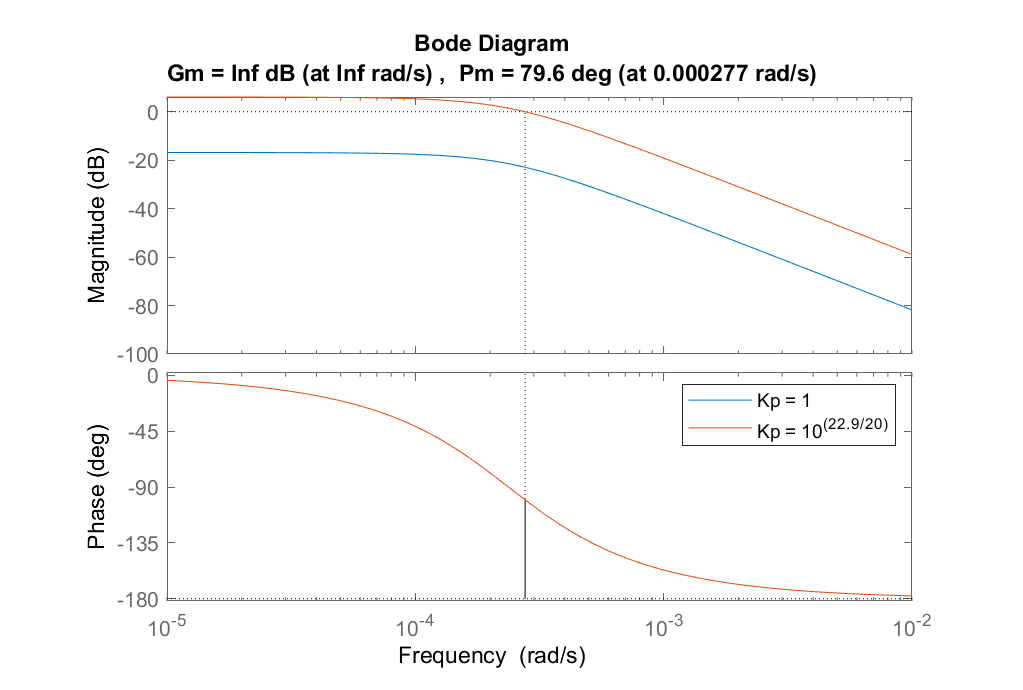
\includegraphics[width=\maxwidth{56.196688409433015em}]{figure_2.eps}
\end{center}


\begin{par}
\begin{flushleft}
\textbf{Proportional kompensering}
\end{flushleft}
\end{par}

\begin{par}
\begin{flushleft}
Der introduceres et proportinal led, som hæver forstærkningen med 22.9 db for at få opnå en 0db knægfrekvens på fasemagenfrekvens (Wpm = 2.625*10\textasciicircum{}-4)
\end{flushleft}
\end{par}

\begin{matlabcode}
Kp = 10^(22.9/20)
\end{matlabcode}
\begin{matlaboutput}
Kp = 13.9637
\end{matlaboutput}
\begin{matlabcode}
margin(Gp*Kp)
\end{matlabcode}
\begin{center}
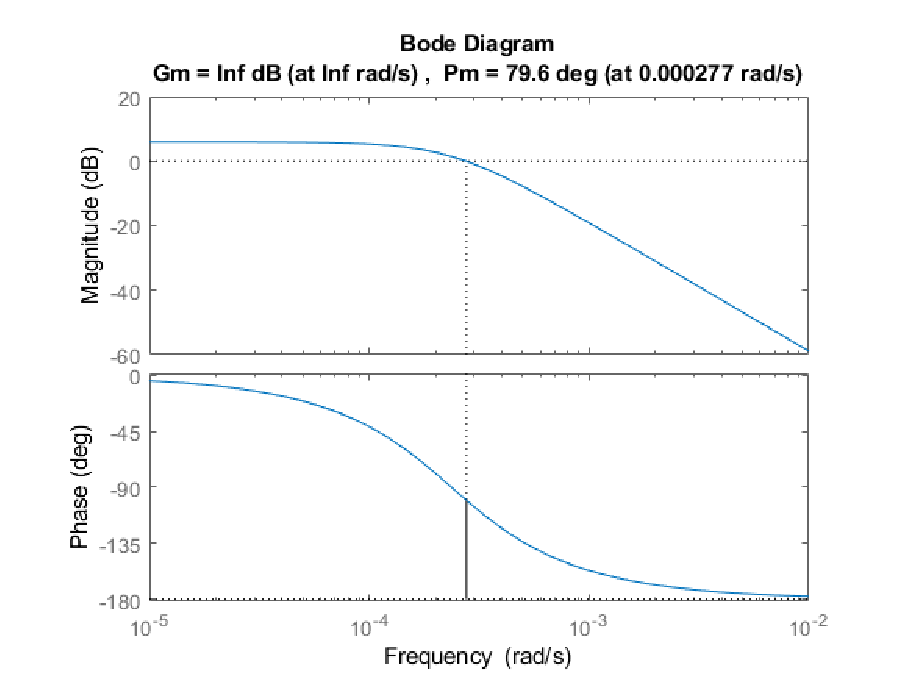
\includegraphics[width=\maxwidth{56.196688409433015em}]{figure_3.eps}
\end{center}

\begin{par}
\begin{flushleft}
Tilføjelsen af Kp resultere i en stationær fejl på 33 procent.
\end{flushleft}
\end{par}

\begin{matlabcode}
DC_Gain = 10^(6.07/20)
\end{matlabcode}
\begin{matlaboutput}
DC_Gain = 2.0114
\end{matlaboutput}
\begin{matlabcode}
ess = 1/(1+DC_Gain)
\end{matlabcode}
\begin{matlaboutput}
ess = 0.3321
\end{matlaboutput}

\begin{par}
\begin{flushleft}
Procent dutycycle forbrug undersøges:
\end{flushleft}
\end{par}

\begin{matlabcode}
step(1.2*feedback(Kp,Gp)+dutycycle_offset)
\end{matlabcode}
\begin{center}
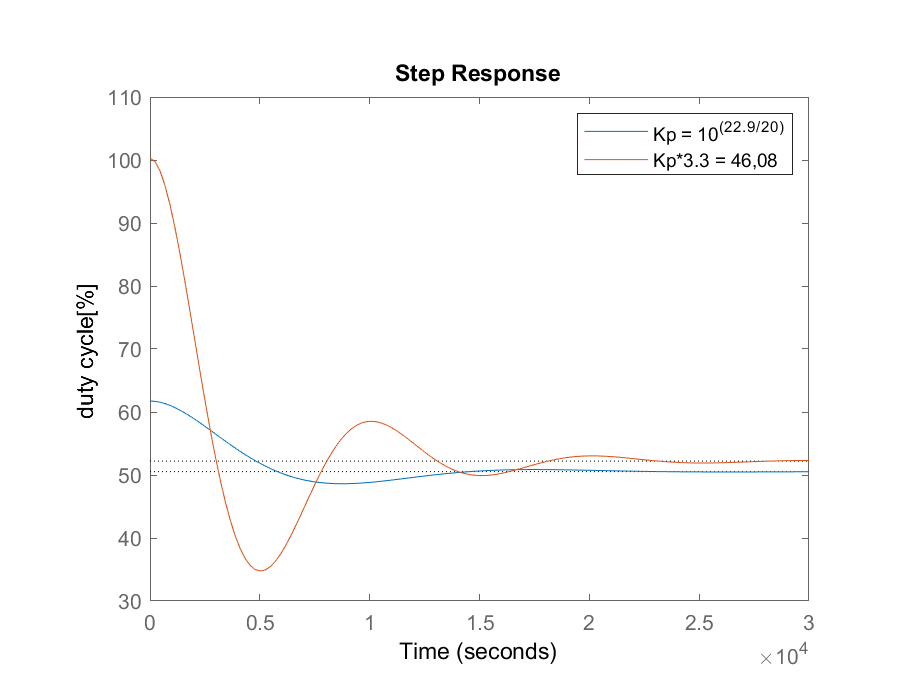
\includegraphics[width=\maxwidth{56.196688409433015em}]{figure_4.eps}
\end{center}

\begin{par}
\begin{flushleft}
Heraf kan det observeres at kun 62\% af den maximale 100\% dutycycle benyttes. 
\end{flushleft}
\end{par}

\begin{par}
\begin{flushleft}
Derfor hæves Kp således 100\% dutycycle benyttes.
\end{flushleft}
\end{par}


\begin{matlabcode}
Kp = 10^(22.9/20)*3.3
\end{matlabcode}
\begin{matlaboutput}
Kp = 46.0802
\end{matlaboutput}
\begin{matlabcode}
step(1.2*feedback(Kp,Gp)+dutycycle_offset)
\end{matlabcode}
\begin{center}
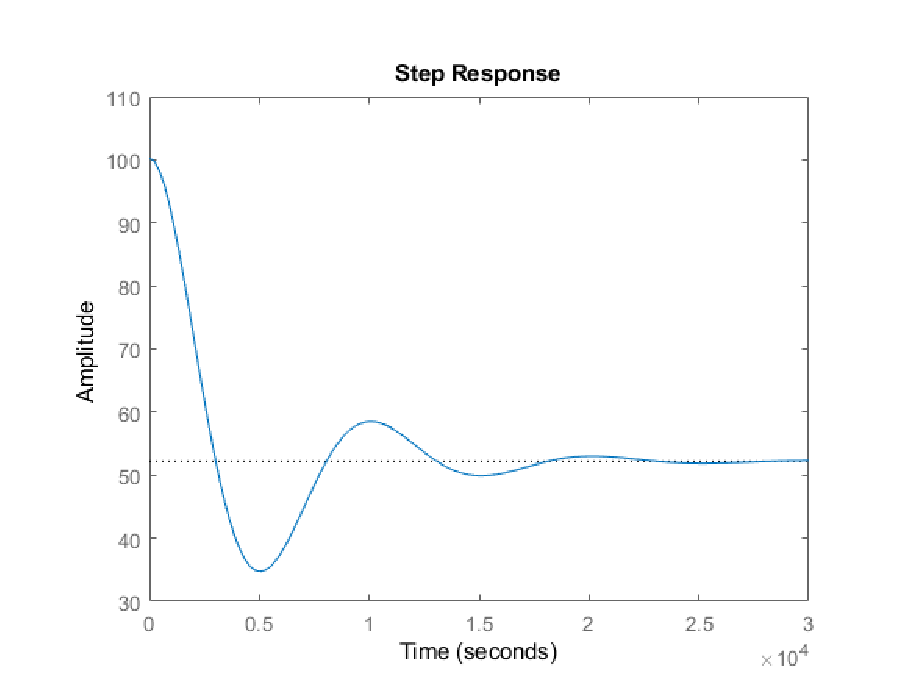
\includegraphics[width=\maxwidth{56.196688409433015em}]{figure_5.eps}
\end{center}

\begin{par}
\begin{flushleft}
Dette giver anledning til en fasemagenfrekvens på 5.88*10\textasciicircum{}-4
\end{flushleft}
\end{par}

\begin{matlabcode}
margin(Gp*Kp)
\end{matlabcode}
\begin{center}
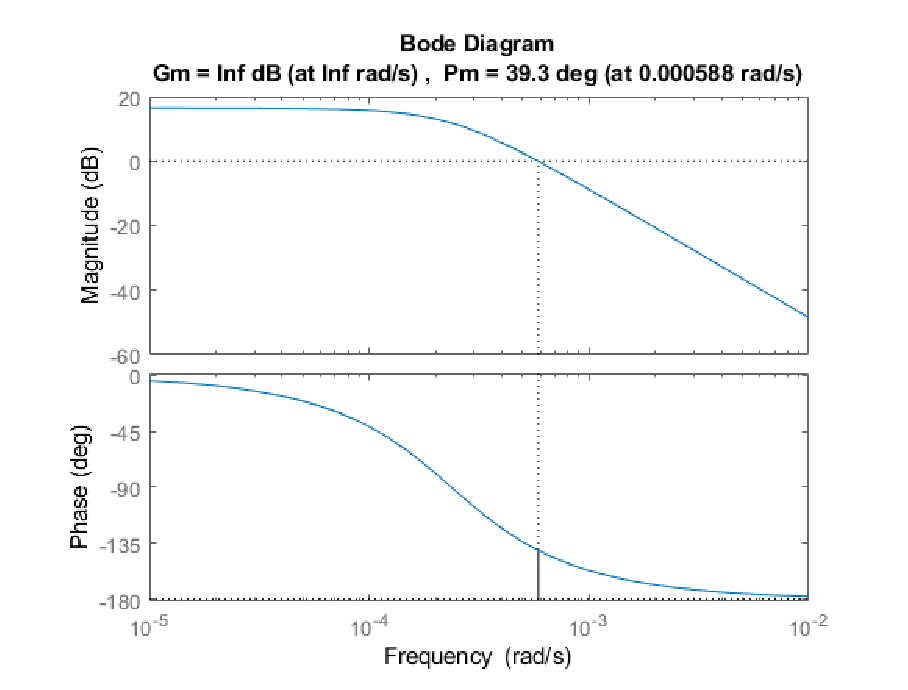
\includegraphics[width=\maxwidth{56.196688409433015em}]{figure_6.eps}
\end{center}
\begin{matlabcode}
Wpm = 5.88*10^-4
\end{matlabcode}
\begin{matlaboutput}
Wpm = 5.8800e-04
\end{matlaboutput}

\begin{par}
\begin{flushleft}
Kp giver giver en mindre stationær fejl. ned til 13\%
\end{flushleft}
\end{par}

\begin{matlabcode}
DC_Gain = 10^(16.46/20)
\end{matlabcode}
\begin{matlaboutput}
DC_Gain = 6.6527
\end{matlaboutput}
\begin{matlabcode}
ess = 100*(1/(1+DC_Gain))
\end{matlabcode}
\begin{matlaboutput}
ess = 13.0672
\end{matlaboutput}


\vspace{1em}
\begin{par}
\begin{flushleft}
Kp kan ikke hæves mere, da de 100\% dutycyle er opnået. Derfor tilføjes en Lag kompensering der kan sikre en stationærfejl på mindre end 1\%
\end{flushleft}
\end{par}


\begin{par}
\begin{flushleft}
\textbf{Lag kompensering}
\end{flushleft}
\end{par}

\begin{matlabcode}
Tlag = 20/Wpm
\end{matlabcode}
\begin{matlaboutput}
Tlag = 3.4014e+04
\end{matlaboutput}

\begin{par}
\begin{flushleft}
Alpha = uendelig, således Lag kan konverteres til et "I" led i en PID model.
\end{flushleft}
\end{par}

\begin{matlabcode}
Glag = (s+(1/Tlag))/(s)
\end{matlabcode}
\begin{matlaboutput}
Glag =
 
  s + 2.94e-05
  ------------
       s
 
Continuous-time transfer function.
\end{matlaboutput}

\begin{par}
\begin{flushleft}
Ud fra bodeplottet af Lag kompenseringne kan de ses at fasenmagnen vil falde 2.9. Dette ses ikke som et problem pt
\end{flushleft}
\end{par}

\begin{matlabcode}
margin(Glag)
\end{matlabcode}
\begin{center}
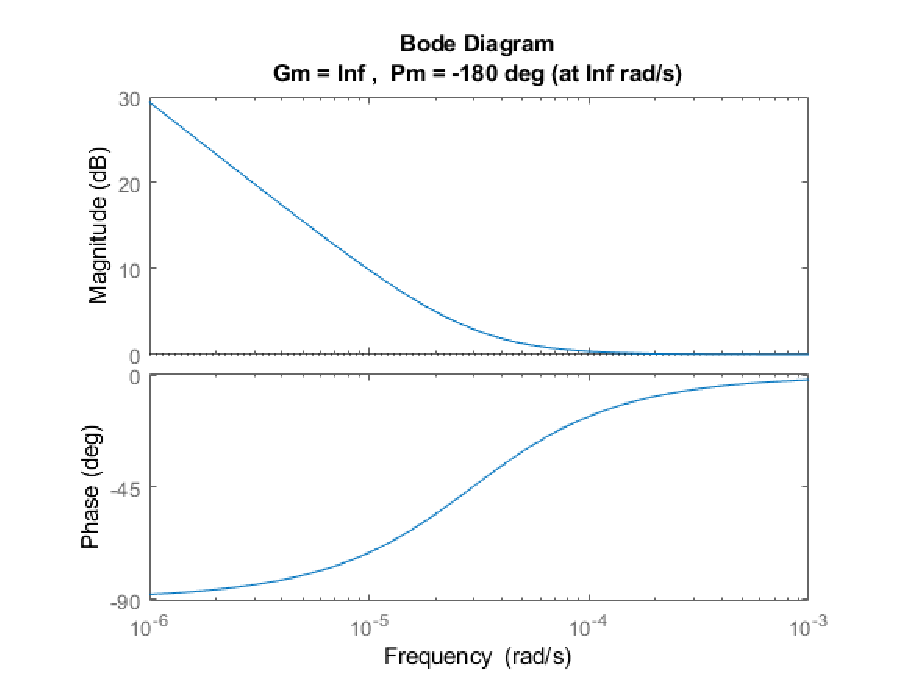
\includegraphics[width=\maxwidth{56.196688409433015em}]{figure_7.eps}
\end{center}

\begin{par}
\begin{flushleft}
DC gain med Lag kompenseringne findes til 45.7 db
\end{flushleft}
\end{par}

\begin{matlabcode}
DC_Gain = 10^(45.7/20)
\end{matlabcode}
\begin{matlaboutput}
DC_Gain = 192.7525
\end{matlaboutput}
\begin{matlabcode}
margin(Glag*Gp*Kp)
\end{matlabcode}
\begin{center}
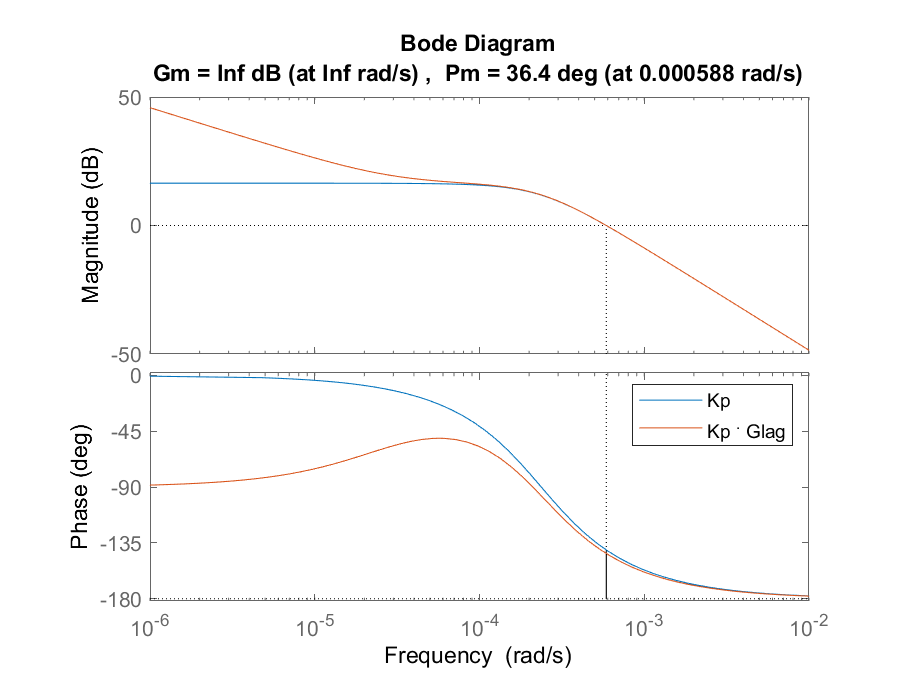
\includegraphics[width=\maxwidth{56.196688409433015em}]{figure_8.eps}
\end{center}

\begin{par}
\begin{flushleft}
Lag regulatoreren ændre den stationære fejl ned til 0.51 procent!
\end{flushleft}
\end{par}

\begin{matlabcode}
100*(1/(1+DC_Gain))
\end{matlabcode}
\begin{matlaboutput}
ans = 0.5161
\end{matlaboutput}

\begin{par}
\begin{flushleft}
Dutycyclen befinder sig stadig i 0-100\% området
\end{flushleft}
\end{par}

\begin{matlabcode}
step(1.2*feedback(Glag*Kp,Gp)+dutycycle_offset)
\end{matlabcode}
\begin{center}
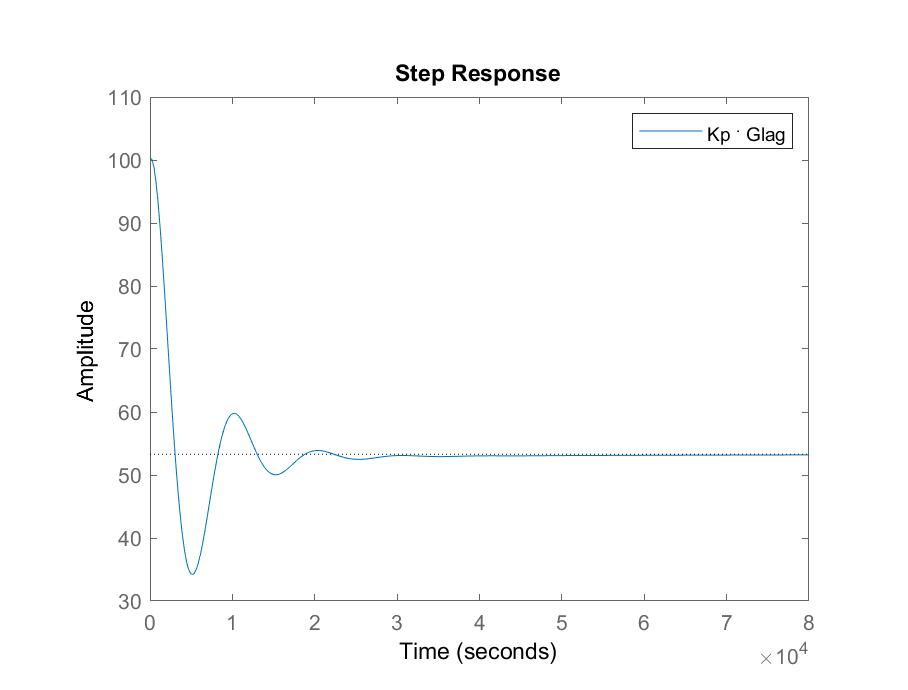
\includegraphics[width=\maxwidth{56.196688409433015em}]{figure_9.eps}
\end{center}


\vspace{1em}

\begin{par}
\begin{flushleft}
\textbf{Steprespons for regulering og proces}
\end{flushleft}
\end{par}

\begin{matlabcode}
step(1.2*feedback(Glag*Kp*Gp,1)+offset_28grader)
\end{matlabcode}
\begin{center}
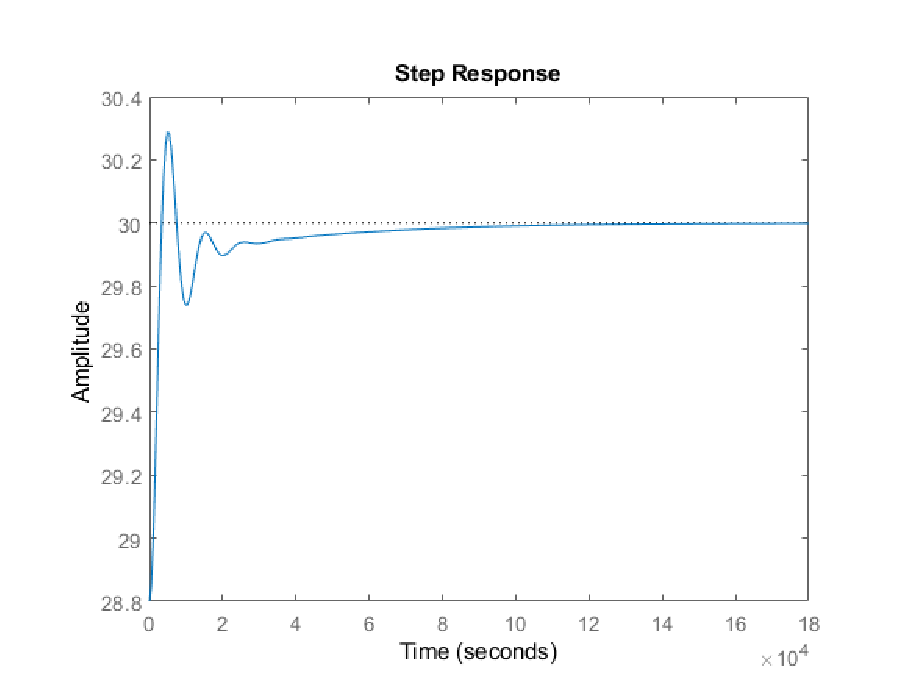
\includegraphics[width=\maxwidth{56.196688409433015em}]{figure_10.eps}
\end{center}
\begin{matlabcode}
S = stepinfo(1.2*feedback(Glag*Kp*Gp,1)+offset_28grader)
\end{matlabcode}
\begin{matlaboutput}
S = 
        RiseTime: 2.2922e+03
    SettlingTime: 6.6068e+04
     SettlingMin: 29.7392
     SettlingMax: 30.2883
       Overshoot: 0.9610
      Undershoot: 0
            Peak: 30.2883
        PeakTime: 4.8886e+03

\end{matlaboutput}

\begin{par}
\begin{flushleft}
Her findes det korteste risetime, regulering af 120W varmelegemet kan udføre. Med et oversving på10\% og et dutycycle forbrug \textless{} 100\%. 
\end{flushleft}
\end{par}


\vspace{1em}
\begin{par}
\begin{flushleft}
\textbf{konklusion}
\end{flushleft}
\end{par}

\begin{enumerate}
\setlength{\itemsep}{-1ex}
   \item{\begin{flushleft} Der skal benyttes en anden taktik for tilføjelsen af væske til akvarie ved for lav vandstand. En taktik hvor vand tilføjes i mindre doser, så reguleringen kan følge med.  \end{flushleft}}
   \item{\begin{flushleft} Der skal benyttes et større varmelegeme der hurtigere kan respondere på varmetabet. se fig (x) for sammenhængen mellem størrelse af varmelegeme med risetime. () \end{flushleft}}
\end{enumerate}

\begin{par}
\begin{flushleft}
\textbf{Valg}
\end{flushleft}
\end{par}

\begin{enumerate}
\setlength{\itemsep}{-1ex}
   \item{\begin{flushleft} Vi fortsætter med varmeligemet på 120 watt og ændre tilføjelsen af væske. \end{flushleft}}
\end{enumerate}


\vspace{1em}

\vspace{1em}

\vspace{1em}


\vspace{1em}
\begin{matlabcode}
Varmelegeme_watt = (60: 60: 6000);
Trise = zeros(1,length(Varmelegeme_watt))
\end{matlabcode}
\begin{matlaboutput}
Trise = 1x100    
     0     0     0     0     0     0     0     0     0     0     0     0     0     0     0     0     0     0     0     0     0     0     0     0     0     0     0     0     0     0     0     0     0     0     0     0     0     0     0     0     0     0     0     0     0     0     0     0     0     0

\end{matlaboutput}
\begin{matlabcode}

for n = 1:length(Varmelegeme_watt)
    Trise(n) = 2292/n;
end
plot(Varmelegeme_watt, Trise)
xlabel('Varmelegeme watt [W]')
ylabel('28.8->30 grader Rise Time. [s]')
xlim([0 2000])
\end{matlabcode}
\begin{center}
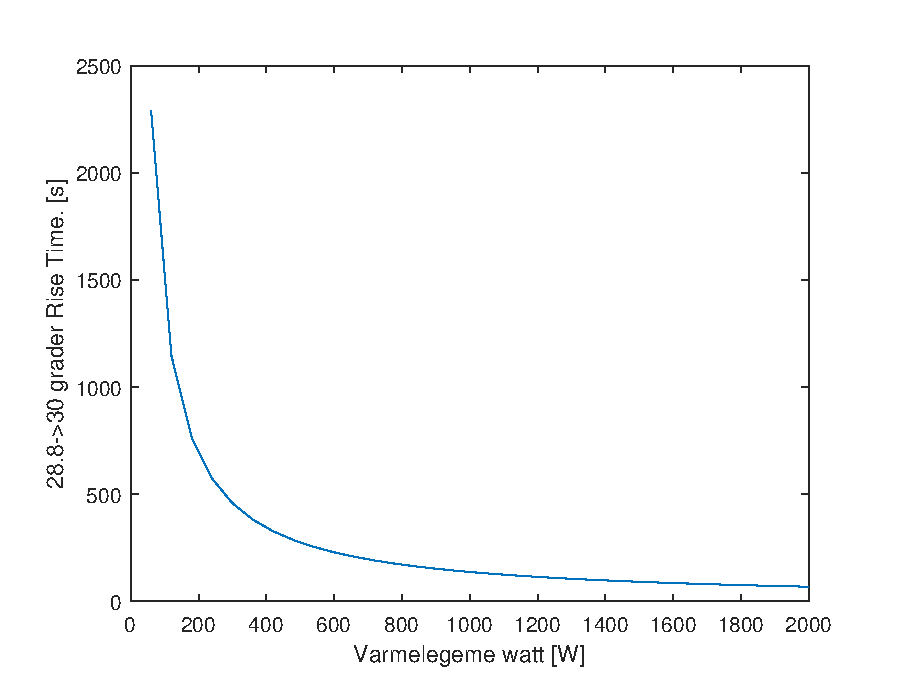
\includegraphics[width=\maxwidth{56.196688409433015em}]{figure_11.eps}
\end{center}

\begin{par}
\begin{flushleft}
Ref til forholdet mellem temperatur ændring, versus watt
\end{flushleft}
\end{par}

\begin{par}
\begin{flushleft}
\href{https://bloglocation.com/art/water-heating-calculator-for-time-energy-power}{https://bloglocation.com/art/water-heating-calculator-for-time-energy-power}
\end{flushleft}
\end{par}


\vspace{1em}


\vspace{1em}
\begin{par}
\begin{flushleft}
\textbf{Diskretisering af regulering og sampling af proces}
\end{flushleft}
\end{par}

\begin{par}
\begin{flushleft}
Ved at sætte samplingtiden på 60 sekunder, er påvirkningne fra diskretiseringen ubetydelig. Dette skyldes systemet er utroligt langsomt 
\end{flushleft}
\end{par}

\begin{par}
\begin{flushleft}
\textbf{Samplingtid = 60 sekunder}
\end{flushleft}
\end{par}

\begin{matlabcode}
Tsample=0.03528/Wpm
\end{matlabcode}
\begin{matlaboutput}
Tsample = 60
\end{matlaboutput}

\begin{par}
\begin{flushleft}
sampling frekven (radianer pr sek til svingning pr sek) 
\end{flushleft}
\end{par}

\begin{matlabcode}
fsample = (2*pi)*(1/Tsample)
\end{matlabcode}
\begin{matlaboutput}
fsample = 0.1047
\end{matlaboutput}
\begin{matlabcode}

\end{matlabcode}

\begin{par}
\begin{flushleft}
sampling af proces
\end{flushleft}
\end{par}

\begin{matlabcode}
Gp_z = c2d(Gp,Tsample,'zoh');
\end{matlabcode}

\begin{par}
\begin{flushleft}
Diskretisering af regulering
\end{flushleft}
\end{par}

\begin{matlabcode}
Gc_z=c2d(Glag*Kp,Tsample,'tustin');
\end{matlabcode}

\begin{par}
\begin{flushleft}
Ændeing ved diskretisering
\end{flushleft}
\end{par}

\begin{matlabcode}
bode(Gp*Glag*Kp)
hold on
margin(Gp_z*Gc_z)
legend ('Kontinuær', 'Diskretiseret')
hold off
\end{matlabcode}
\begin{center}
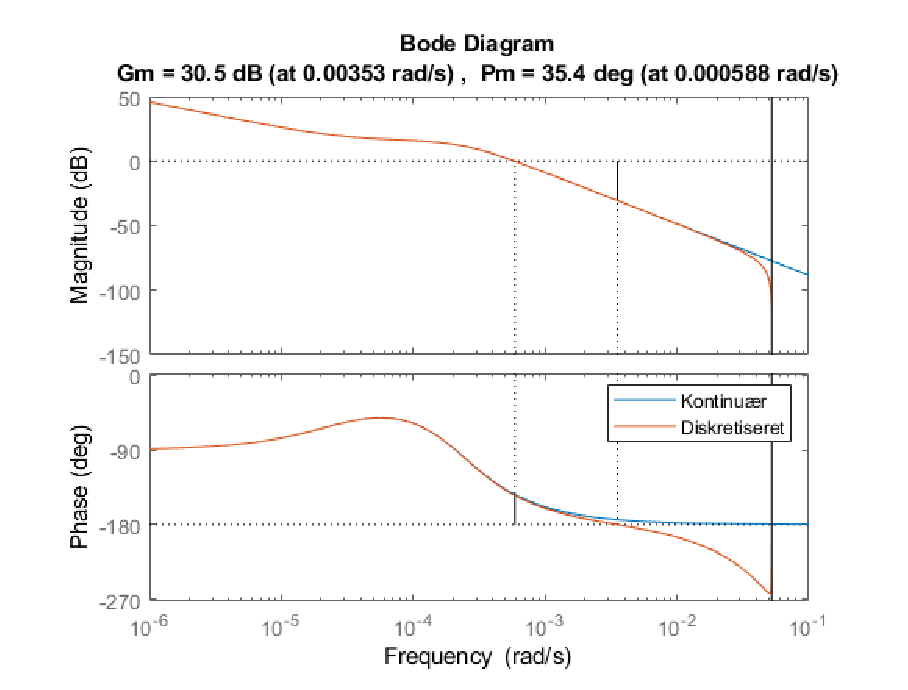
\includegraphics[width=\maxwidth{56.196688409433015em}]{figure_12.eps}
\end{center}
\begin{matlabcode}

step(1.2*feedback(Gp*Glag*Kp,1)+offset_28grader)
hold on
step(1.2*feedback(Gp_z*Gc_z,1)+offset_28grader)
title 'step 1.2 grader [C{\circ}], kontinuær vs diskretisering'
xlabel('Tid [s]')
ylabel('Tempertur [C{\circ}]')
legend ('Kontinuær', 'Diskretiseret')
hold off
\end{matlabcode}
\begin{center}
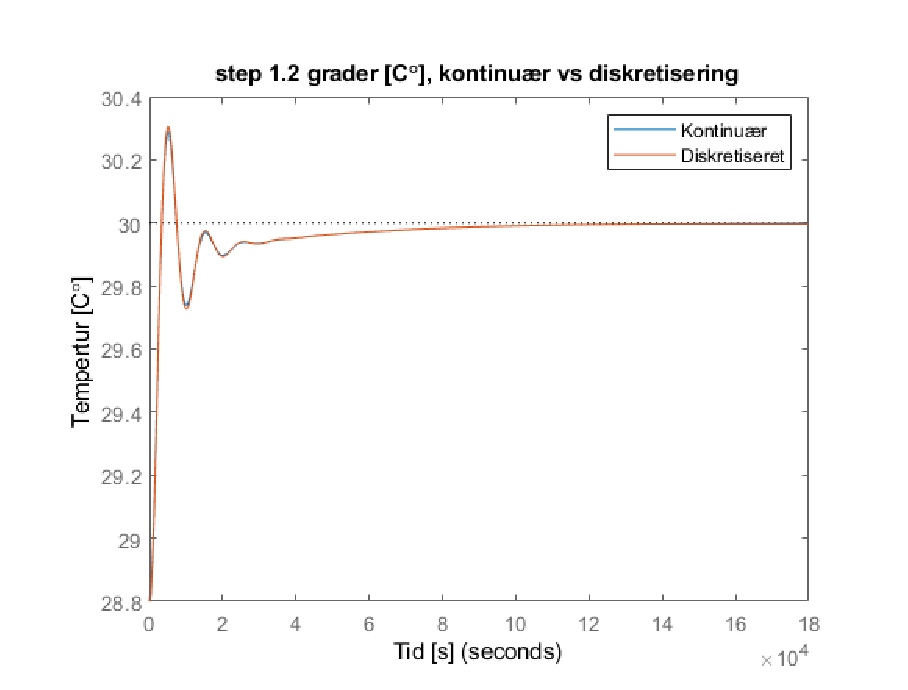
\includegraphics[width=\maxwidth{56.196688409433015em}]{figure_13.eps}
\end{center}
\begin{matlabcode}

step(1.2*feedback(Glag*Kp,Gp)+dutycycle_offset)
hold on
step(1.2*feedback(Gc_z,Gp_z)+dutycycle_offset)
title 'step 1.2 grader [C{\circ}], kontinuær vs diskretisering, dutycycle'
xlabel('Tid [s]')
ylabel('dutycycle [%]')
legend ('Kontinuær', 'Diskretiseret')
hold off
\end{matlabcode}
\begin{center}
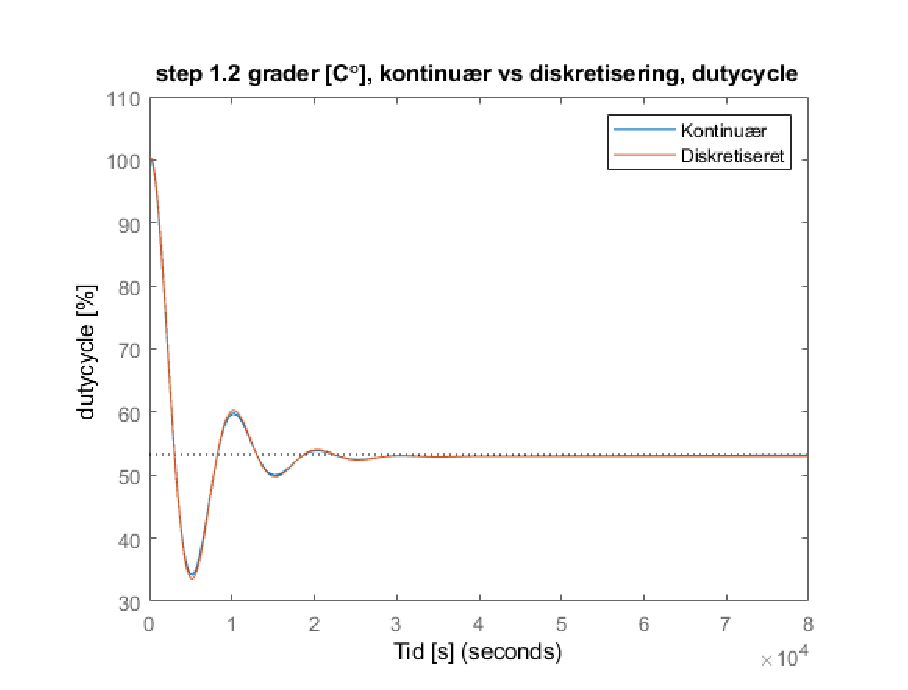
\includegraphics[width=\maxwidth{56.196688409433015em}]{figure_14.eps}
\end{center}



\vspace{1em}
\begin{par}
\begin{flushleft}
\textbf{Konvertingen fra Proportional-Lag regulator, til PI regulator}
\end{flushleft}
\end{par}

\begin{par}
\begin{flushleft}
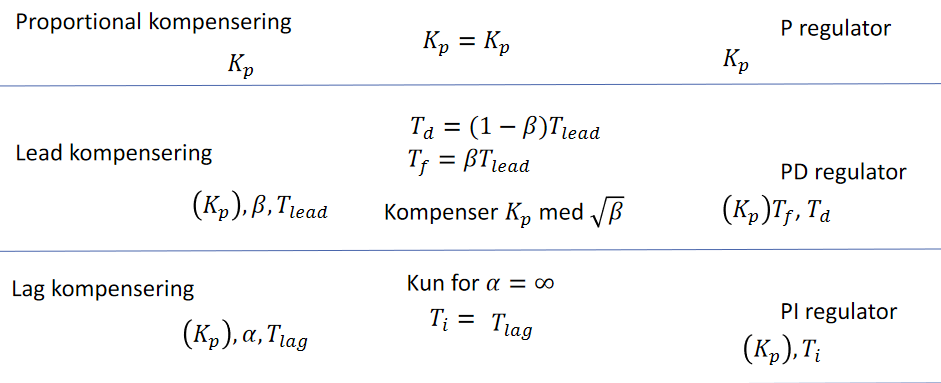
\includegraphics[width=\maxwidth{53.98896136477672em}]{image_2}
\end{flushleft}
\end{par}

\begin{par}
\begin{flushleft}
Ti = Tlag = 3.4014*10\textasciicircum{}-4
\end{flushleft}
\end{par}

\begin{par}
\begin{flushleft}
Kp = 46.0802
\end{flushleft}
\end{par}


\vspace{1em}
\begin{par}
\begin{flushleft}
PI Kopling
\end{flushleft}
\end{par}

\begin{par}
\begin{flushleft}
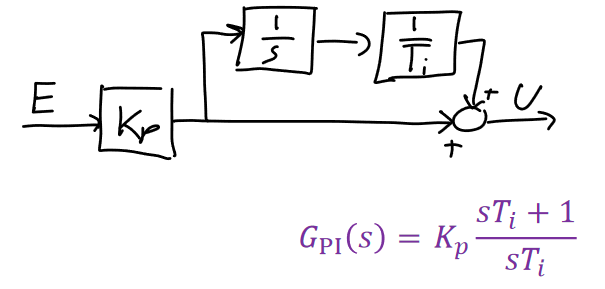
\includegraphics[width=\maxwidth{42.24786753637732em}]{image_3}
\end{flushleft}
\end{par}


\vspace{1em}
\begin{par}
\begin{flushleft}
\textbf{Diskretisering af integrator }
\end{flushleft}
\end{par}

\begin{par}
\begin{flushleft}
Benyttes bilinærtransformation 
\end{flushleft}
\end{par}

\begin{par}
\begin{flushleft}
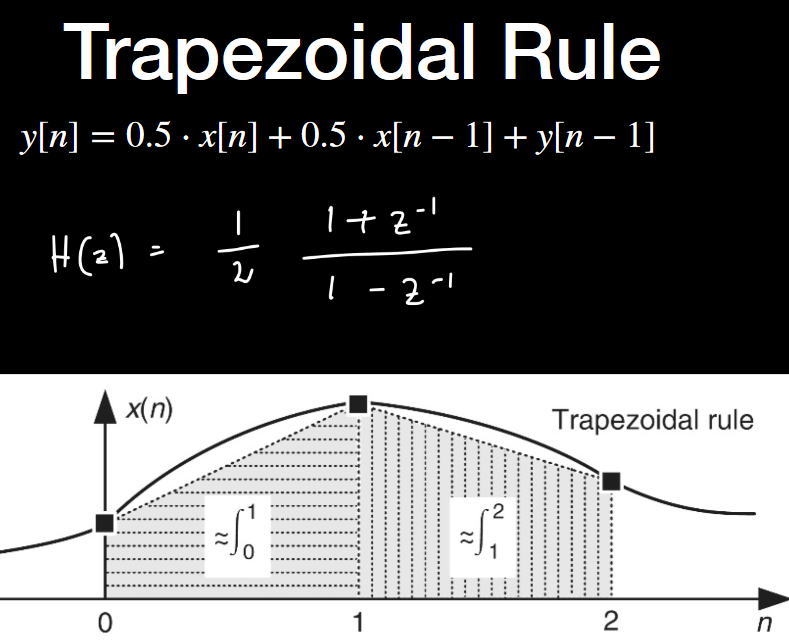
\includegraphics[width=\maxwidth{45.55945810336177em}]{image_4}
\end{flushleft}
\end{par}


\vspace{1em}
\begin{par}
\begin{flushleft}
integration i kontinuær tid = 1/s
\end{flushleft}
\end{par}

\begin{par}
\begin{flushleft}
proportional kompensering i kontinuær tid = Kp
\end{flushleft}
\end{par}


\vspace{1em}
\begin{par}
\begin{flushleft}
diskretisering af integration med bilinærtransformaiton = (1/2)*(1+z\textasciicircum{}-1)/(1-z\textasciicircum{}-1)
\end{flushleft}
\end{par}

\begin{par}
\begin{flushleft}
diskretisering af proportional kompensering = Kp
\end{flushleft}
\end{par}


\vspace{1em}


\vspace{1em}
\begin{par}
\begin{flushleft}
differensligning af integrator:
\end{flushleft}
\end{par}

\begin{par}
\begin{flushleft}
Y(Z)/X(Z) = (1/2)*(1+z\textasciicircum{}-1)/(1-z\textasciicircum{}-1)
\end{flushleft}
\end{par}

\begin{par}
\begin{flushleft}
Y(Z)*(1-z\textasciicircum{}-1) = (1/2)*(1+z\textasciicircum{}-1)*X(Z)
\end{flushleft}
\end{par}

\begin{par}
\begin{flushleft}
Y(Z) = (1/2)*X(Z)+ (1/2)*X(Z)*z\textasciicircum{}-1+Y(Z)*z\textasciicircum{}-1
\end{flushleft}
\end{par}

\begin{par}
\begin{flushleft}
y(n) = (1/2)*x(n)+(1/2)*x(n-1)*y(n-1)
\end{flushleft}
\end{par}

\begin{matlabcode}
%y(n) = (1/2)*x(n)+(1/2)*x(n-1)*y(n-1)
\end{matlabcode}
\begin{matlaboutput}
Unrecognized function or variable 'x'.
\end{matlaboutput}

\begin{par}
\begin{flushleft}
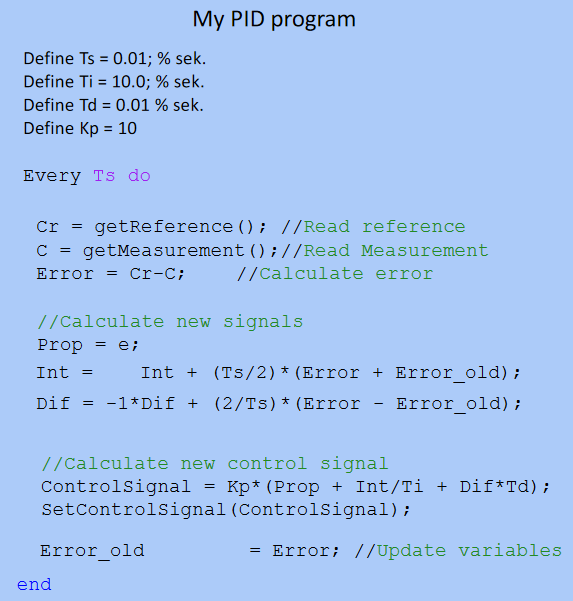
\includegraphics[width=\maxwidth{43.853487205218265em}]{image_5}
\end{flushleft}
\end{par}

\begin{par}
\begin{flushleft}
Definering af hvorfor integralledet ser sådan ud
\end{flushleft}
\end{par}

\begin{par}
\begin{flushleft}
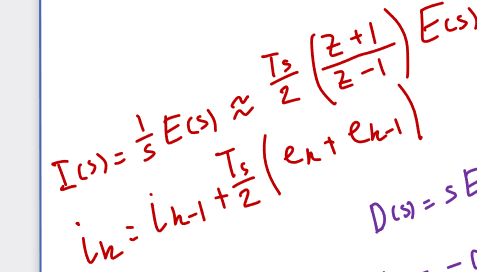
\includegraphics[width=\maxwidth{47.867536377320626em}]{image_6}
\end{flushleft}
\end{par}


\vspace{1em}

\vspace{1em}

\begin{par}
\begin{flushleft}
Rate limiter - rampe begrænser
\end{flushleft}
\end{par}

\begin{par}
\begin{flushleft}
25 -\textgreater{} 30
\end{flushleft}
\end{par}

\begin{par}
\begin{flushleft}
step 0.1 -\textgreater{} regulator
\end{flushleft}
\end{par}

\begin{par}
\begin{flushleft}
vent 10 min
\end{flushleft}
\end{par}

\begin{par}
\begin{flushleft}
25.1 -\textgreater{} 30
\end{flushleft}
\end{par}

\begin{par}
\begin{flushleft}
step 0.1 -\textgreater{} regulator
\end{flushleft}
\end{par}

\begin{par}
\begin{flushleft}
25.2 -\textgreater{} 30
\end{flushleft}
\end{par}

\begin{par}
\begin{flushleft}
vent 10 min ......
\end{flushleft}
\end{par}


\vspace{1em}
\begin{par}
\begin{flushleft}
integrator logik, max 100\% 
\end{flushleft}
\end{par}

\begin{par}
\begin{flushleft}
PI 
\end{flushleft}
\end{par}

\begin{par}
\begin{flushleft}
Opdater ikke integral, hvis control isgnal er under 100\% (anti Winde up)
\end{flushleft}
\end{par}

\begin{matlabcode}

\end{matlabcode}

\end{document}
